\section{Analyse af problemområde}

Ud fra systemdefinitionen ved vi at systemet skal holde styr på følgende:

\begin{itemize}
	\item Tilbud
	\item Varer
	\item Opskrifter
\end{itemize}

Med disse informationer kan systemet hjælpe brugeren til at finde billige varer i bestemte butikker, og eventuelt anbefale opskrifter der bruger disse tilbudsvarer.
I de følgende afsnit vil disse emner blive beskrevet vha. klassebeskrivelser, en hændelsestabel, og et klassediagram.

\subsection{Klasser}
For at kunne håndtere de 3 allerede nævnte klasser, tilbud, varer og opskrifter, skal der være flere for at danne en sammenhæng.
Denne sammenhæng vil analyseres her.

\textbf{Vare:}
En vare indgår i opskrifter, og indkøbslister.
Når man laver sin indkøbsliste kan man vælge varer man vil købe, og tilføje dem til indkøbslisten.
Desuden kan en vare have et antal tilbud hver uge, hvilket betyder at der også skal laves en tilbudsklasse.

\textbf{Tilbud:}
Hver uge kommer der nye varer på tilbud fra de fleste danske dagligvarebutikker.
Disse modeleres og kobles på varen og dermed dannes der en kobling fra varen til tilbudene.

\textbf{Opskrift:}
En opskrift har en liste over ingredienser, hvilket altså er varer, samt mængden af varen.
I interviewene i \myref{section:interview2}, blev det nævnt at brugerne gerne ville kunne vurdere en opskrift, og dermed få anbefalet yderligere opskrifter som minder om denne.
Dette leder til at der laves en såkaldt vurderingsklasse.

\textbf{Vurdering:}
Vurderinger bliver foretaget når en bruger af systemet har udført en opskrift, og vil give den en vurdering, både til at hjælpe andre, men også for at få lignende opskrifter anbefalet, hvis en bruger fandt en opskrift god.

\textbf{Anbefaling:}
En anbefaling, af en opskrift, kan gives til personer når de har givet positive vurderinger af andre opskrifter, som minder om den vurderede opskrift.

\textbf{Person:}
Personklassen gør det muligt at hold styr på forskellige personer, da disse tilsluttes andre aspekter af systemet.
Disse er opskrifter og vurderinger.
Derudover vil en person også have præferencer som vil være attributter.

\textbf{Indkøbsliste:}
Indkøbslisten laves af en person, og fyldes op med objekter fra vareklassen.
Indkøbslisterne kan deles mellem flere brugere, og derfor skal koblingen på personenklassen ikke være singulær, men altså 1..*.

\subsection{Hændelser}
Vi har fundet frem til de forskellige hændelser der sker i problemområdet.
Ud fra disse laves en hændelsestabel, der beskriver hvilke klasser forskellige hændelser påvirker.
Formålet med at identificere hændelserne samt at analysere disse i en hændelsestalbel, er at forstå problemområdet bedre og dermed hjælpe med forståelsen for hvordan en løsning ville kunne designes for at afhjælpe de problemer der findes i problemområdet. Desuden kan tabellen hjælpe med strukturen på klasserne.
Hvis to klasser har samme hændelser, kan disse klasser ofte tilpasses under en klasse og dermed opnå en bedre struktur.

\begin{table}[H]
  \centering
    \colorlet{shadecolor}{gray!40}
    \rowcolors{1}{white}{shadecolor}
      \begin{tabular}{l|lccccccc}
      %\hline
       								& \rot{Tilbud}  & \rot{Indkøbsliste} & \rot{Opskrift} & \rot{Vare} & \rot{Person}& \rot{Vurderinger} \\ \hline
      Vare tilføjet til indkøbsliste&               & +      &          & +     & +     &   \\ 
      Vare fjernet fra indkøbsliste	&              	& +      &          & +     & +     &   \\ 
      Vare aftjekket på indkøbsliste&               & +      &          & +     & +     &   \\ 
      Opskrift valgt ???       		& +             & +      &          & +     & +     &   \\ 
      Tilbud oprettet        		& +            	& +      & +        & +     &       &   \\ 
      Tilbud aktiveret        		& +            	& +      & +        & +     &       &   \\ 
      Tilbud udgået          		& +        		& +      & +     	&       &       &   \\ 
      Vare tilføjet til overvågning & +          	&        &          & +     & +     &   \\ 
      Vare fjernet fra overvågning  & +          	&        &          & +     & +     &   \\ 
      Overvågningsvare på tilbud    & +  			&		 &			& + 	& +		&	\\
      Del indkøbsliste       		&               & +      &          &       & +     &   \\ 
      Indkøbsliste oprettet  		&              	& +      &          &       & +     &   \\ 
      Indkøbsliste slettet  		&             	& +      &          &       & +     &   \\ 
      Vurdering givet				&             	&        & +        &       & +		& + \\
      Anbefaling givet				&				&		 & +		&		& +		& + \\
      
    \end{tabular}
  \caption{Hændelsestabel. Viser hvilket klasser, problemområdets hændelser påvirker.}\label{tabel:haendelsestabel}
\end{table}


Hændelsestabellen i \myref{tabel:haendelsestabel} viser både hvilke hændelser der findes i problemområdet, samt hvilke klasser de påvirker.
Hvis tabellen læses vandret kan det ses at klasser der bliver påvirket af mange hændelser er klasser som ``Indkøbsliste'', ``Vare'' og ``Person''.

Ud fra analysen indtil nu kan der dannes et overblik, over klassernes interne interaktion, såvel som hvilke hændelser der involverer hvilke klasser.
Denne information kan vi nu bruge til at lave en struktur over klasserne i problemområdet.

\subsection{Struktur}\label{sec:struktur}
\begin{figure}
	\centering
		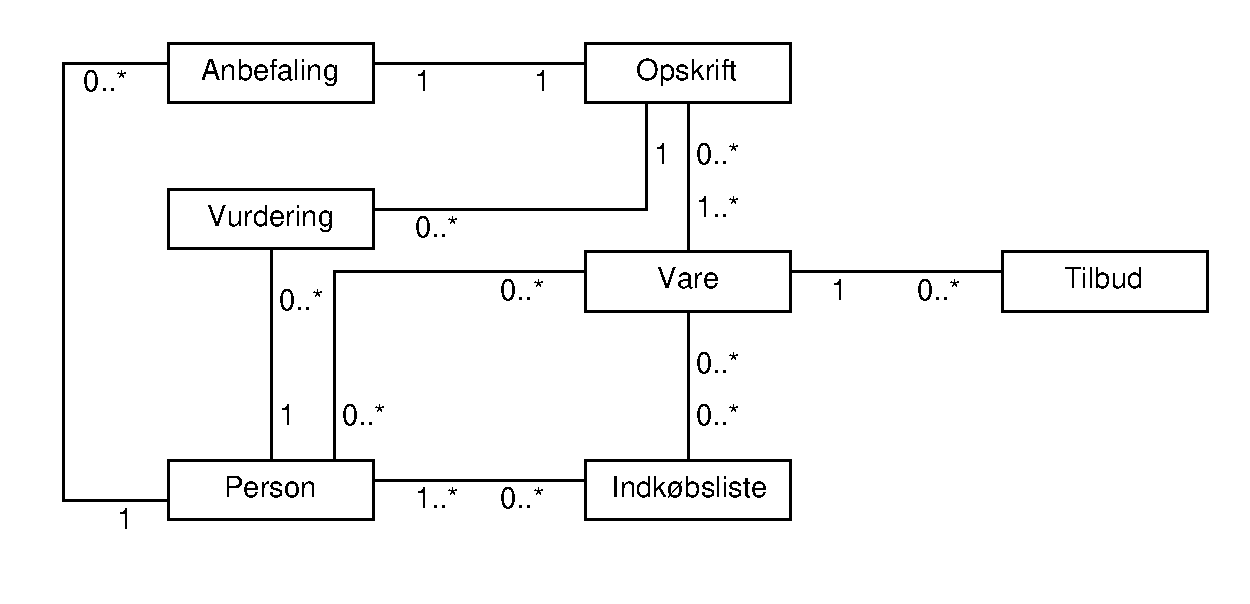
\includegraphics[scale=0.6]{images/Diagrams/klassediagram_model_simple.pdf}
	\caption{Klassediagram over problemområdet.}
	\label{figur:PDklasse}
\end{figure}

Klassediagram som ses på \myref{figur:PDklasse}, dette beskriver forholdet mellem de forskellige klasser som findes i problemområdet.
Diagrammets sammenhænge er dannet ud fra hændelsestabellen, og beskrivelserne af klasserne.
Følgende afsnit gennemgår diagrammets sammenhænge.

Personer i indkøbssituationer kan lave indkøbslister, disse indkøbslister kan været ejet og administreret af en enten en eller flere personer.
En indkøbsliste kan bestå af nul til mange varer.
En vare kan være på tilbud i mere end en butik, og derfor have nul til mange tilbud.
En vare kan desuden indgå i en opskrift, og er derfor forbundet med nul til mange.
Desuden har opskrifterne en til mange varer på listen over ingredienser.
Varen kan også være tilføjet til overvågningslisten hos en person, så derfor har personer og varer en nul til mange relation på hinanden.
En person i problemområdet kan give hver opskrift en vurdering, derfor kan personen give nul til mange vurderinger.
En vurdering gives til en opskrift alene, imens en opskrift kan have mange vurderinger, eller ingen vurderinger.
Anbefalinger består af en opskrift, imens personen kan modtage nul til mange anbefalinger.

%På baggrund af denne analyse kan systemets implementation designes, men først skal der foretages en analyse af anvendelsesområdet.
Ovenstående analyse vil hjælpe til at designe systemets implementering, først foretages dog en analyse af anvendelsesområdet, for at undersøge hvad der er muligt at foretage sig i systemet.
